\documentclass[11pt,a4paper]{article}

\usepackage[T1]{fontenc}
\usepackage[utf8]{inputenc}
% Se sul sistema e' installato il pacchetto lingua italiano (italian.ldf) viene
% usato babel; altrimenti si ripiega su nomi italiani e sillabazione disattivata.
\IfFileExists{italian.ldf}{%
  \usepackage[italian]{babel}%
}{%
  \usepackage[none]{hyphenat}%
  \renewcommand{\figurename}{Figura}%
  \renewcommand{\tablename}{Tabella}%
  \renewcommand{\contentsname}{Indice}%
  \renewcommand{\abstractname}{Sommario}%
  \renewcommand{\refname}{Riferimenti bibliografici}%
  \sloppy\emergencystretch=3em
}
\usepackage[margin=25mm]{geometry}
\usepackage{amsmath,amssymb}
\usepackage{siunitx}
\usepackage{booktabs}
\usepackage{graphicx}
\usepackage{circuitikz}
\usepackage{tikz}
\usepackage{caption}
\usepackage{enumitem}
\usepackage[hidelinks]{hyperref}

\sisetup{per-mode=symbol, detect-weight=true, range-phrase={ a }, range-units=single}
\ctikzset{bipoles/length=0.9cm}

\title{Linee Guida di Progetto per Driver di Gate per Tiristori\\[2mm]
\large Requisiti, compromessi e circuiti di esempio per applicazioni a controllo\\ di fase e commutate dalla rete}
\author{}
\date{}

\begin{document}
\maketitle

\begin{abstract}
\noindent
Questa nota raccoglie i requisiti pratici che governano il progetto di un driver di
gate (unità di gate) per tiristori a controllo di fase e commutati dalla rete, dai
piccoli dispositivi a vite fino ai grandi SCR press-pack impiegati in raddrizzatori
e soft starter di classe \si{\mega\watt}. Vengono esaminate per prime la
caratteristica gate--catodo e i limiti di datasheet, poi i requisiti su ampiezza,
pendenza, durata dell'impulso e polarizzazione a riposo. Seguono isolamento,
alimentazione ausiliaria, protezioni, layout e diagnostica. Sono infine proposte e
discusse quattro topologie rappresentative di driver, con un esempio numerico
svolto per un dispositivo press-pack da
\SI{6.5}{\kilo\volt}/\SI{2.6}{\kilo\ampere}. Il documento si chiude con una
checklist di progetto.
\end{abstract}

\tableofcontents

%======================================================================
\section{Scopo e Terminologia}
%======================================================================

L'oggetto di questa nota è l'\emph{unità di gate}: il circuito elettronico che
converte un comando di accensione a livello logico, riferito alla massa del
controllo, in un impulso di corrente di gate riferito al catodo di un tiristore
flottante al potenziale di rete.

Tre funzioni sono sempre presenti e vanno progettate separatamente:

\begin{enumerate}[label=(\roman*)]
  \item \textbf{Isolamento del segnale} --- trasferire il comando di accensione
        attraverso la barriera di isolamento senza distorsione e con adeguata
        immunità ai transitori di modo comune.
  \item \textbf{Erogazione di energia} --- fornire la carica di gate con ampiezza,
        pendenza e durata richieste.
  \item \textbf{Protezione e controllo dello stato di interdizione} --- mantenere il
        dispositivo saldamente spento in assenza di comando e impedire accensioni
        spurie.
\end{enumerate}

La nota è scritta per \emph{tiristori a controllo di fase} (PCT) e per
\emph{tiristori rapidi/inverter-grade}, che vengono spenti dalla commutazione del
circuito. I dispositivi a spegnimento comandato da gate (GTO, IGCT) sono fuori
ambito: richiedono un percorso di spegnimento a bassissima induttanza,
concettualmente diverso, trattato da letteratura dedicata. I tiristori a innesco
ottico (LTT) sono citati solo dove rilevanti per la discussione sull'isolamento.

%======================================================================
\section{Il Gate: Comportamento Fisico e Parametri di Datasheet}
%======================================================================

\subsection{La giunzione gate--catodo}

Elettricamente, il percorso gate--catodo è una giunzione $p$--$n$ di grande area,
fortemente interdigitata, derivata dalla struttura distribuita di cortocircuiti di
emettitore del catodo. Si comporta quindi come un diodo in parallelo a una
resistenza, con caratteristica $I_G$--$V_G$ fortemente non lineare e ampia
dispersione da esemplare a esemplare. \emph{Non} è un carico capacitivo come il
gate di un MOSFET o di un IGBT: il driver deve erogare corrente sostenuta, non solo
carica.

L'innesco avviene quando la corrente di gate iniettata porta il guadagno di corrente
della sezione $npn$ al punto di soddisfare la condizione rigenerativa
$\alpha_{pnp}+\alpha_{npn}\ge 1$ nella regione adiacente al gate. La conduzione poi
si \emph{propaga lateralmente} da quella regione con velocità dell'ordine di
\SIrange{50}{100}{\micro\metre\per\micro\second}. Questo fenomeno di propagazione è
la ragione fisica per cui la forma dell'impulso di gate, e non solo la sua ampiezza,
determina il $\mathrm{d}i/\mathrm{d}t$ di anodo tollerabile.

\subsection{Il diagramma di innesco}

I parametri di datasheet che definiscono la caratteristica di uscita richiesta al
driver sono:

\begin{description}[style=nextline,leftmargin=2.2cm,labelwidth=2cm]
  \item[$V_{GT}$, $I_{GT}$] Tensione e corrente di innesco di gate: i valori che
        garantiscono l'accensione, specificati a \SI{25}{\celsius} e spesso anche a
        $T_{vj,\min}$.
  \item[$V_{GD}$, $I_{GD}$] Tensione e corrente di non innesco: i valori al di sotto
        dei quali il dispositivo è garantito \emph{non} accendersi, specificati a
        $T_{vj,\max}$. L'uscita del driver a riposo deve restare sotto questi valori
        con margine.
  \item[$I_L$, $I_H$] Corrente di latching e di mantenimento. L'impulso di gate deve
        durare finché la corrente di anodo non ha superato $I_L$.
  \item[$V_{FGM}$, $I_{FGM}$] Tensione e corrente di picco diretta di gate.
  \item[$V_{RGM}$] Tensione inversa di picco di gate --- tipicamente solo
        \SIrange{5}{10}{\volt}. È il limite più frequentemente violato nella
        pratica.
  \item[$P_{GM}$, $P_{G(AV)}$] Potenza di gate dissipabile di picco e media,
        quest'ultima solitamente specificata su una finestra di
        \SI{20}{\milli\second}.
\end{description}

Riportando questi limiti sul piano $V_G$--$I_G$ si ottiene il classico diagramma di
innesco di Fig.~\ref{fig:trigger}. La regola di progetto è semplice da enunciare:

\begin{quote}
\emph{La retta di carico del driver di gate, tracciata sul diagramma di innesco,
deve passare interamente nell'area di ``accensione certa'' su tutto il campo di
temperatura di funzionamento, e non deve mai oltrepassare i limiti $P_{GM}$,
$V_{FGM}$ o $I_{FGM}$.}
\end{quote}

\begin{figure}[htbp]
\centering
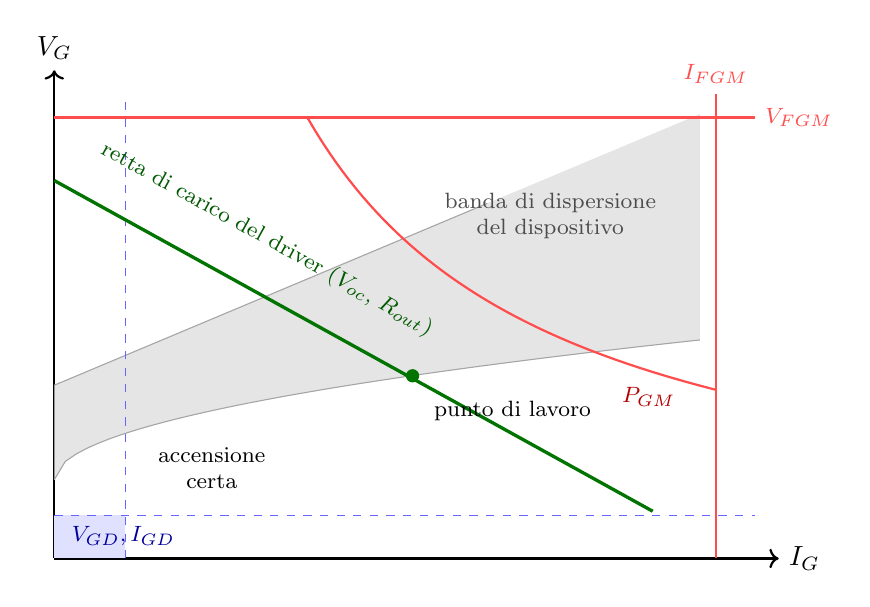
\begin{tikzpicture}[scale=1.0]
  % axes
  \draw[->,thick] (0,0) -- (9.2,0) node[right] {$I_G$};
  \draw[->,thick] (0,0) -- (0,6.2) node[above] {$V_G$};

  % device characteristic spread band
  \fill[gray!20]
    plot[domain=0:8.2,samples=60] (\x,{1.0+0.62*sqrt(\x)})
    -- (8.2,{2.2+0.42*8.2}) -- plot[domain=8.2:0,samples=60] (\x,{2.2+0.42*\x})
    -- cycle;
  \draw[gray!70] plot[domain=0:8.2,samples=60] (\x,{1.0+0.62*sqrt(\x)});
  \draw[gray!70] plot[domain=0:5.5,samples=60] (\x,{2.2+0.42*\x});
  \node[gray!60!black,align=center,font=\footnotesize]
    at (6.3,4.35) {banda di dispersione\\del dispositivo};

  % non-trigger region
  \fill[blue!12] (0,0) rectangle (0.9,0.55);
  \draw[blue!60,dashed] (0.9,0) -- (0.9,5.9);
  \draw[blue!60,dashed] (0,0.55) -- (8.9,0.55);
  \node[blue!60!black,font=\footnotesize,anchor=west] at (0.05,0.28)
    {\,$V_{GD},I_{GD}$};

  % max limits
  \draw[red!70,thick] (8.4,0) -- (8.4,5.9) node[above,font=\footnotesize] {$I_{FGM}$};
  \draw[red!70,thick] (0,5.6) -- (8.9,5.6) node[right,font=\footnotesize] {$V_{FGM}$};
  % power hyperbola  V*I = 18
  \draw[red!70,thick] plot[domain=3.22:8.4,samples=60] (\x,{18/\x});
  \node[red!70!black,font=\footnotesize] at (7.55,2.05) {$P_{GM}$};

  % driver load line
  \draw[very thick,green!45!black] (0,4.8) -- (7.6,0.6);
  \node[green!35!black,font=\footnotesize,rotate=-29] at (2.7,4.05)
    {retta di carico del driver ($V_{oc}$, $R_{out}$)};
  \fill[green!45!black] (4.55,2.32) circle (2.4pt);
  \node[font=\footnotesize,anchor=north west] at (4.7,2.12) {punto di lavoro};

  % certain firing region label
  \node[align=center,font=\footnotesize] at (2.0,1.15)
    {accensione\\certa};
\end{tikzpicture}
\caption{Diagramma di innesco del gate di un tiristore. La retta di carico del
driver deve intersecare la banda di dispersione del dispositivo all'interno
dell'area di accensione certa e restare al di sotto dei limiti $P_{GM}$, $V_{FGM}$ e
$I_{FGM}$. La regione blu è l'area di non innesco garantito a $T_{vj,\max}$.}
\label{fig:trigger}
\end{figure}

\subsection{Temperatura e dispersione}

Due effetti dominano il dimensionamento:

\begin{itemize}
  \item $I_{GT}$ \textbf{aumenta a bassa temperatura}, tipicamente di un fattore
        \numrange{2}{4} tra \SI{25}{\celsius} e \SI{-40}{\celsius}, perché i
        cortocircuiti di emettitore deviano una frazione maggiore della corrente di
        gate quando la vita dei portatori è bassa. \textbf{Il driver va dimensionato
        a $T_{vj,\min}$}, cioè per l'avviamento a freddo, non alla temperatura
        nominale di giunzione.
  \item $V_{GD}$ e $I_{GD}$ \textbf{diminuiscono ad alta temperatura}. Il margine di
        interdizione va quindi verificato a $T_{vj,\max}$.
\end{itemize}

La dispersione di $I_{GT}$ tra esemplari dello stesso tipo di produzione è
comunemente un fattore tre o più. Progettare sul valore tipico è un guasto in campo
garantito; il punto di partenza corretto è il massimo di datasheet alla minima
temperatura di funzionamento.

%======================================================================
\section{Requisiti sull'Impulso di Gate}
%======================================================================

\subsection{Ampiezza: hard firing}

Il requisito minimo è $I_G > I_{GT}(T_{vj,\min})$, ma non viene mai usato nella
pratica. La regola di progetto accettata è

\begin{equation}
  I_{G,\text{peak}} \;\ge\; 3 \dots 10 \times I_{GT}\big(T_{vj,\min}\big),
  \label{eq:amp}
\end{equation}

con l'estremo superiore dell'intervallo usato ogni volta che ci si attende un
elevato $\mathrm{d}i/\mathrm{d}t$ di anodo. La ragione è il meccanismo di
propagazione laterale: una corrente di gate elevata accende un'area di catodo
iniziale più grande, quindi la densità di corrente iniziale --- e con essa la
dissipazione locale nei primi microsecondi --- è più bassa. Il valore di
$\mathrm{d}i/\mathrm{d}t$ dichiarato a datasheet è \emph{sempre} condizionato a un
pilotaggio di gate specificato; un pilotaggio più debole lo invalida.

Per grandi dispositivi press-pack è tipico un $I_{G,\text{peak}}$ nell'intervallo
\SIrange{2}{5}{\ampere}, a fronte di valori di $I_{GT}$ di poche centinaia di
milliampere.

\subsection{Pendenza}

La velocità di salita della corrente di gate è importante quanto l'ampiezza:

\begin{equation}
  \frac{\mathrm{d}i_G}{\mathrm{d}t} \;\ge\; \SI{1}{\ampere\per\micro\second}
  \quad \text{(tip.\ \SIrange{1}{5}{\ampere\per\micro\second} per hard drive).}
  \label{eq:didt}
\end{equation}

Equivalentemente, un tempo di salita $t_r < \SI{1}{\micro\second}$, e preferibilmente
\SIrange{0.1}{0.5}{\micro\second}, misurato \emph{ai morsetti del dispositivo} e non
all'uscita del driver. È questa la specifica che vincola l'induttanza del loop di
gate:

\begin{equation}
  L_{loop} \;\le\; \frac{V_{drive} - V_{GT} - R_G I_G}{\mathrm{d}i_G/\mathrm{d}t}.
  \label{eq:lloop}
\end{equation}

Con un doppino intrecciato di circa \SI{1}{\micro\henry\per\metre}, questo limita
immediatamente la lunghezza pratica del cavo tra unità di gate e dispositivo.

\subsection{Durata, latching e back porch}

L'impulso deve persistere finché la corrente di anodo non ha superato con margine la
corrente di latching $I_L$. Vanno distinti tre casi:

\begin{itemize}
  \item \textbf{Carico resistivo, impulso breve.} Un impulso di
        \SIrange{20}{100}{\micro\second} è adeguato.
  \item \textbf{Carico induttivo.} La corrente di anodo sale lentamente; l'impulso
        richiesto può andare da centinaia di microsecondi a diversi millisecondi. Un
        impulso troppo breve provoca mancate accensioni intermittenti, tipicamente
        solo a basso carico --- un classico problema di messa in servizio.
  \item \textbf{Conduzione discontinua, percorsi di ricircolo, connessione
        serie/parallelo.} L'approccio più sicuro è mantenere il gate pilotato per
        tutto l'intervallo di conduzione atteso.
\end{itemize}

La forma d'onda standard è quindi un \emph{impulso hard seguito da un back porch}
(Fig.~\ref{fig:pulse}): un picco breve e di ampiezza elevata che garantisce
un'accensione rapida e su area estesa, seguito da un plateau basso di
$1\dots2\times I_{GT}$ che mantiene il dispositivo acceso fino a latching certo,
contenendo la dissipazione media di gate entro $P_{G(AV)}$.

\begin{figure}[htbp]
\centering
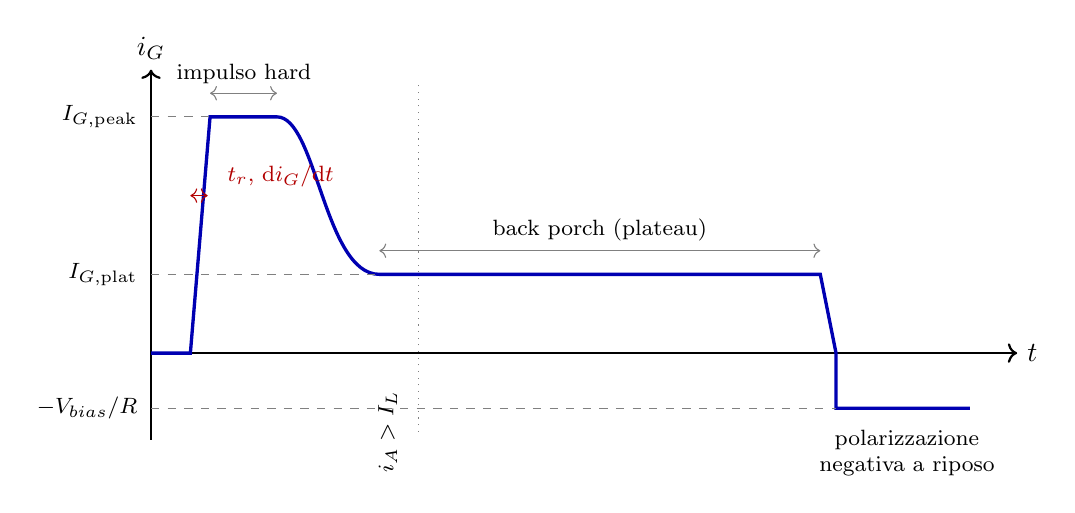
\begin{tikzpicture}[xscale=1.0,yscale=1.0]
  \draw[->,thick] (0,0) -- (11,0) node[right] {$t$};
  \draw[->,thick] (0,-1.1) -- (0,3.6) node[above] {$i_G$};

  % waveform
  \draw[very thick,blue!70!black]
    (0,0) -- (0.5,0) -- (0.75,3.0) -- (1.6,3.0)
    .. controls (2.1,3.0) and (2.2,1.0) .. (2.9,1.0)
    -- (8.5,1.0) -- (8.7,0) -- (8.7,-0.7) -- (10.4,-0.7);

  % annotations
  \draw[<->,gray] (0.75,3.3) -- (1.6,3.3);
  \node[font=\footnotesize,anchor=south] at (1.18,3.3) {impulso hard};
  \draw[<->,gray] (2.9,1.3) -- (8.5,1.3);
  \node[font=\footnotesize,anchor=south] at (5.7,1.3) {back porch (plateau)};
  \draw[dashed,gray] (0,3.0) -- (0.75,3.0);
  \node[font=\footnotesize,anchor=east] at (-0.05,3.0) {$I_{G,\text{peak}}$};
  \draw[dashed,gray] (0,1.0) -- (2.9,1.0);
  \node[font=\footnotesize,anchor=east] at (-0.05,1.0) {$I_{G,\text{plat}}$};
  \draw[dashed,gray] (0,-0.7) -- (8.7,-0.7);
  \node[font=\footnotesize,anchor=east] at (-0.05,-0.7) {$-V_{bias}/R$};
  \node[font=\footnotesize,anchor=north,align=center] at (9.6,-0.85)
    {polarizzazione\\negativa a riposo};
  % rise time
  \draw[<->,red!70!black] (0.5,2.0) -- (0.72,2.0);
  \node[font=\footnotesize,anchor=west,red!70!black] at (0.85,2.25)
    {$t_r$, $\mathrm{d}i_G/\mathrm{d}t$};
  % latching
  \draw[dotted,gray] (3.4,-1.0) -- (3.4,3.4);
  \node[font=\footnotesize,anchor=south,rotate=90] at (3.25,-1.0)
    {$i_A > I_L$};
\end{tikzpicture}
\caption{Forma d'onda raccomandata per la corrente di gate: impulso iniziale hard
per un'accensione rapida e su area estesa, back porch che mantiene il dispositivo
fino al latching, polarizzazione negativa (o nulla) nello stato di interdizione.}
\label{fig:pulse}
\end{figure}

\subsection{Polarizzazione a riposo e immunità al \texorpdfstring{$\mathrm{d}v/\mathrm{d}t$}{dv/dt}}

Quando il tiristore è interdetto ma polarizzato direttamente, la corrente di
spostamento attraverso la capacità della giunzione di blocco,
$i = C_j\,\mathrm{d}v/\mathrm{d}t$, fluisce in parte nella regione di gate e può
innescare il dispositivo. Contromisure, in ordine di efficacia:

\begin{enumerate}
  \item Una \textbf{resistenza gate--catodo} $R_{GK}$ montata \emph{sul
        dispositivo}, tipicamente \SIrange{10}{100}{\ohm} per dispositivi grandi e
        fino a \SI{1}{\kilo\ohm} per quelli piccoli. Devia dal gate la corrente di
        spostamento e la corrente di perdita della giunzione. Carica anche il
        driver, e di questo va tenuto conto nel dimensionamento.
  \item Una \textbf{polarizzazione negativa di gate} di \SIrange{-2}{-5}{\volt} tra
        un impulso e il successivo. È la soluzione più robusta ma richiede uno
        stadio di uscita bipolare e deve rispettare $V_{RGM}$ con margine,
        oscillazioni incluse.
  \item Uno \textbf{stato di riposo a bassa impedenza}: lo stadio di uscita deve
        presentare al gate una bassa impedenza quando è inattivo, non un'alta
        impedenza.
\end{enumerate}

Si noti che progetto dello snubber e immunità al $\mathrm{d}v/\mathrm{d}t$ sono
accoppiati: un'unità di gate non può compensare uno snubber RC inadeguato.

\subsection{Riepilogo dei valori obiettivo}

\begin{table}[htbp]
\centering
\caption{Valori obiettivo tipici per un driver di gate di tiristore a controllo di
fase. I valori di datasheet prevalgono sempre su queste indicazioni.}
\label{tab:targets}
\begin{tabular}{@{}llp{6.4cm}@{}}
\toprule
\textbf{Grandezza} & \textbf{Obiettivo tipico} & \textbf{Osservazioni} \\
\midrule
$I_{G,\text{peak}}$ & $3\dots10\times I_{GT}(T_{\min})$ &
  Estremo superiore per alto $\mathrm{d}i/\mathrm{d}t$ \\
$\mathrm{d}i_G/\mathrm{d}t$ & \SIrange{1}{5}{\ampere\per\micro\second} &
  Misurato ai morsetti del dispositivo \\
$t_r$ & \SIrange{0.1}{1}{\micro\second} & Fissa il budget di induttanza del loop \\
Durata impulso hard & \SIrange{10}{50}{\micro\second} & Copre ritardo di accensione e propagazione \\
$I_{G,\text{plat}}$ & $1\dots2\times I_{GT}$ & Limitato da $P_{G(AV)}$ \\
Durata del plateau & fino a $i_A > I_L$ &
  Tutto l'intervallo di conduzione con carichi induttivi \\
Polarizzazione a riposo & da \SI{0}{\volt} a \SI{-5}{\volt} &
  Mai oltre $V_{RGM}$, oscillazioni incluse \\
$R_{GK}$ & \SIrange{10}{100}{\ohm} & Montata sul dispositivo, non sul driver \\
Jitter & $< \SI{1}{\micro\second}$ &
  Critico per stack in serie e ripartizione di corrente \\
Ritardo comando--gate & allineato entro \SI{1}{\micro\second} &
  Tra tutti i canali di un ponte \\
\bottomrule
\end{tabular}
\end{table}

%======================================================================
\section{Isolamento e Coordinamento dell'Isolamento}
%======================================================================

L'unità di gate attraversa la barriera di isolamento principale del convertitore, e
la sua tenuta va derivata dallo stesso studio di coordinamento del resto
dell'apparecchiatura (IEC 60664-1, IEC 61800-5-1 per gli azionamenti), considerando:

\begin{itemize}
  \item la \textbf{tensione di modo comune a regime} del catodo rispetto alla massa
        di controllo;
  \item i livelli di \textbf{picco ripetitivo} e di \textbf{tenuta a impulso} (BIL)
        dell'impianto;
  \item \textbf{distanze superficiali e in aria} per il grado di inquinamento e
        l'altitudine del sito;
  \item la \textbf{tensione di innesco delle scariche parziali} per apparecchiature
        in media tensione, che di norma governa il progetto del trasformatore di
        isolamento ben prima della tenuta dielettrica;
  \item l'\textbf{immunità ai transitori di modo comune} (CMTI), cioè il
        $\mathrm{d}v/\mathrm{d}t$ che la barriera vede durante la commutazione. La
        capacità di accoppiamento attraverso la barriera, $C_{io}$, inietta
        $i = C_{io}\,\mathrm{d}v/\mathrm{d}t$ nell'elettronica di controllo.
        Minimizzare $C_{io}$ (schermo elettrostatico tra gli avvolgimenti, fibra
        ottica) è la difesa principale.
\end{itemize}

Si usano tre strategie di isolamento:

\begin{table}[htbp]
\centering
\caption{Confronto tra le strategie di isolamento del comando di accensione.}
\label{tab:iso}
\begin{tabular}{@{}p{3.1cm}p{4.6cm}p{4.6cm}@{}}
\toprule
\textbf{Strategia} & \textbf{Vantaggi} & \textbf{Limiti} \\
\midrule
Trasformatore d'impulso &
  Trasporta insieme comando ed energia; nessuna alimentazione locale; semplice,
  robusto, collaudato &
  Il limite volt$\cdot$secondo vincola la durata dell'impulso; l'induttanza di
  dispersione limita $\mathrm{d}i_G/\mathrm{d}t$; serve il reset del nucleo;
  $C_{io}$ dell'ordine dei \si{\pico\farad} \\
\addlinespace
Optoaccoppiatore + alimentazione isolata &
  Durata dell'impulso arbitraria; sagomatura semplice; basso costo &
  Isolamento tipicamente limitato a pochi \si{\kilo\volt}; il CMTI è un vincolo di
  progetto; richiede un'alimentazione ausiliaria isolata \\
\addlinespace
Fibra ottica + alimentazione locale &
  Isolamento praticamente illimitato; $C_{io}$ trascurabile; ideale per stack in
  serie e per la MT &
  Richiede una sorgente di energia locale (trasformatore ausiliario o
  autoalimentazione); più componenti; gestione e invecchiamento della fibra \\
\bottomrule
\end{tabular}
\end{table}

Per gli stack in serie la fibra ottica è di fatto obbligatoria, sia per il livello di
isolamento sia perché il ritardo di trasmissione deve essere allineato tra tutti i
livelli entro il microsecondo, per evitare ripartizioni di tensione disuniformi
durante l'accensione.

%======================================================================
\section{Alimentazione Ausiliaria dell'Unità di Gate}
%======================================================================

L'unità di gate consuma, per ogni accensione, un'energia dell'ordine di

\begin{equation}
  E_{fire} \approx V_G I_{G,\text{peak}} t_{hard} + V_G I_{G,\text{plat}} t_{plat},
\end{equation}

che per un dispositivo grande vale pochi millijoule --- poco in termini assoluti, ma
deve essere disponibile con bassa impedenza di sorgente per soddisfare la
Eq.~\eqref{eq:didt}. Le opzioni sono:

\begin{enumerate}
  \item \textbf{Convertitore DC/DC isolato} con trasformatore ad alto isolamento che
        alimenta il lato flottante. Soluzione diretta, ma il trasformatore diventa il
        componente critico per l'isolamento e la sua capacità tra avvolgimenti
        degrada direttamente il CMTI.
  \item \textbf{Avvolgimento ausiliario sul trasformatore principale} o
        trasformatore di potenziale dedicato di piccola potenza, comune nei grandi
        raddrizzatori a controllo di fase.
  \item \textbf{Autoalimentazione dalla tensione anodo--catodo}, prelevando energia
        durante l'intervallo di blocco attraverso una resistenza serie di alta
        tensione o, in modo più efficiente, dalla corrente dello snubber RC. Elimina
        completamente la barriera per il percorso di potenza, ma richiede una
        gestione attenta dell'avviamento, poiché prima dell'energizzazione del
        convertitore non è disponibile energia.
  \item \textbf{Condensatore di accumulo locale} dimensionato per diversi impulsi
        consecutivi, così che la corrente d'impulso venga prelevata dal condensatore
        e non dall'alimentazione. È questo, in pratica, a determinare il
        $\mathrm{d}i_G/\mathrm{d}t$ ottenibile: il condensatore va posto
        immediatamente allo stadio di uscita.
\end{enumerate}

%======================================================================
\section{Proposte Circuitali}
%======================================================================

Vengono proposte quattro topologie, in ordine crescente di prestazioni e costo.

\subsection{Circuito A --- Trasformatore d'impulso con rete di peaking}

È la soluzione di riferimento per dispositivi singoli e impulsi da brevi a medi
(Fig.~\ref{fig:circA}). Un MOSFET low-side applica la tensione ausiliaria al
primario del trasformatore. Il condensatore di blocco DC $C_b$ realizza il reset
automatico del nucleo e blocca qualunque componente continua dovuta a un driver
bloccato in conduzione, che altrimenti saturerebbe il nucleo distruggendo il MOSFET.

Sul secondario, la rete di peaking sagoma la forma d'onda a due livelli di
Fig.~\ref{fig:pulse}: sul fronte di salita $C_p$ cortocircuita $R_p$, quindi la
corrente di gate è limitata dal solo $R_s$ e il valore di picco è elevato; man mano
che $C_p$ si carica, la corrente si assesta sul valore di plateau fissato da
$R_s + R_p$. Equazioni di progetto:

\begin{align}
  I_{G,\text{peak}} &\approx \frac{n V_{cc} - V_{GT} - V_{D}}{R_s},
  &
  I_{G,\text{plat}} &\approx \frac{n V_{cc} - V_{GT} - V_{D}}{R_s + R_p}
      - \frac{V_{GT}}{R_{GK}},
  \label{eq:peak}\\[1mm]
  \tau_p &= C_p\,\big(R_p \parallel R_s\big),
  &
  t_{hard} &\approx 3\tau_p ,
\end{align}

dove $n$ è il rapporto spire e $V_D$ la caduta del diodo serie di blocco $D_s$. La
capacità volt$\cdot$secondo del nucleo fissa la massima durata dell'impulso:

\begin{equation}
  A_e \;\ge\; \frac{V_{cc}\, t_{pulse}}{N_1 \Delta B}.
  \label{eq:volt-sec}
\end{equation}

\begin{figure}[htbp]
\centering
\begin{circuitikz}[american]
  % ---------- primary side ----------
  \draw (0.0,6.4) node[left,font=\small]{$+V_{cc}$} -- (1.0,6.4);
  \draw (1.0,6.4) to[C, l_=$C_{st}$, *-] (1.0,3.2) node[ground]{};
  \draw (1.0,6.4) to[C, l=$C_b$] (2.6,6.4);
  \draw (2.6,6.4) -- (5.0,6.4);
  \draw (3.4,6.4) to[zzD, l_=$D_z$, *-] (3.4,3.6);
  \draw (3.4,3.6) -- (4.2,3.6);
  % transformer
  \node[transformer core] (T) at (5.8,5.0) {};
  \draw (5.0,6.4) -| (T.A1);
  \draw (T.A2) -| (4.2,3.6);
  % primary switch
  \node[nigfete, anchor=D] (M) at (4.2,3.6) {};
  \fill (4.2,3.6) circle (1.6pt);
  \draw (M.S) -- (4.2,1.9) node[ground]{};
  \draw (M.G) -- ++(-0.3,0) to[R, l_=$R_g$] ++(-0.6,0)
        node[left,font=\scriptsize]{comando};
  % isolation barrier
  \draw[dashed,gray] (5.8,1.9) -- (5.8,4.1);
  \draw[dashed,gray] (5.8,5.9) -- (5.8,7.9);
  \node[gray!50!black,font=\footnotesize] at (5.8,1.5) {barriera di isolamento};
  % ---------- secondary side ----------
  \draw (T.B1) -| (7.2,6.4);
  \draw (7.2,6.4) to[D, l=$D_s$] (8.4,6.4);
  \draw (8.4,6.4) to[R, l=$R_s$] (9.7,6.4);
  \draw (10.0,6.4) to[R, l_=$R_p$] (11.4,6.4);
  \draw (9.7,6.4) -- (10.0,6.4);
  \draw (10.0,6.4) -- (10.0,7.5) to[C, l=$C_p$] (11.4,7.5) -- (11.4,6.4);
  \draw (11.4,6.4) -- (13.4,6.4);
  % return conductor
  \draw (T.B2) -| (7.2,2.6);
  \draw (7.2,2.6) -- (13.9,2.6);
  % network at the device terminals
  \draw (11.9,6.4) to[R, l_=$R_{GK}$, *-*] (11.9,2.6);
  \draw (12.9,6.4) to[zzD, *-*] (12.9,2.6);
  \node[font=\footnotesize] at (12.9,6.85) {$D_{tvs}$};
  % thyristor
  \draw (13.9,7.9) node[above,font=\footnotesize]{A} -- (13.9,7.4);
  \draw (13.9,7.4) to[Ty, mirror, n=Th, l=$Th$] (13.9,3.4);
  \draw (13.9,3.4) -- (13.9,2.0) node[below,font=\footnotesize]{K};
  \draw (Th.G) -| (13.4,6.4);
  \fill (13.9,2.6) circle (1.6pt);
\end{circuitikz}
\caption{Circuito A --- driver di gate a trasformatore d'impulso con condensatore di
blocco DC $C_b$ per il reset del nucleo, clamp $D_z$ al primario e rete di peaking
$R_s$/$R_p$/$C_p$ al secondario, che produce la forma d'onda impulso hard più back
porch. $R_{GK}$ e il TVS sono montati ai morsetti del dispositivo.}
\label{fig:circA}
\end{figure}

\paragraph{Note.}
\begin{itemize}
  \item Il diodo serie $D_s$ impedisce la corrente inversa di gate durante il reset
        del nucleo e protegge il gate dall'escursione negativa; senza di esso
        $V_{RGM}$ viene facilmente superata.
  \item L'induttanza di dispersione del trasformatore compare in serie al loop di
        gate e limita direttamente il $\mathrm{d}i_G/\mathrm{d}t$. È necessario un
        avvolgimento bifilare o interlacciato; ma l'interlacciamento aumenta
        $C_{io}$, quindi i due requisiti vanno bilanciati esplicitamente.
  \item Il condensatore di accumulo locale $C_{st}$ va posto al primario del
        trasformatore, con area di loop minima verso il MOSFET.
\end{itemize}

\subsection{Circuito B --- Driver chopped (a treno d'impulsi)}

La Eq.~\eqref{eq:volt-sec} rende costosi gli impulsi lunghi: un impulso di
\SI{500}{\micro\second} a \SI{24}{\volt} richiede un nucleo circa venti volte più
grande di uno da \SI{25}{\micro\second}. La soluzione standard è \emph{spezzettare}
l'impulso a \SIrange{5}{20}{\kilo\hertz} (Fig.~\ref{fig:circB}). Il trasformatore
vede allora solo i volt$\cdot$secondo di un periodo di portante, mentre l'inviluppo
può essere lungo a piacere.

\begin{figure}[htbp]
\centering
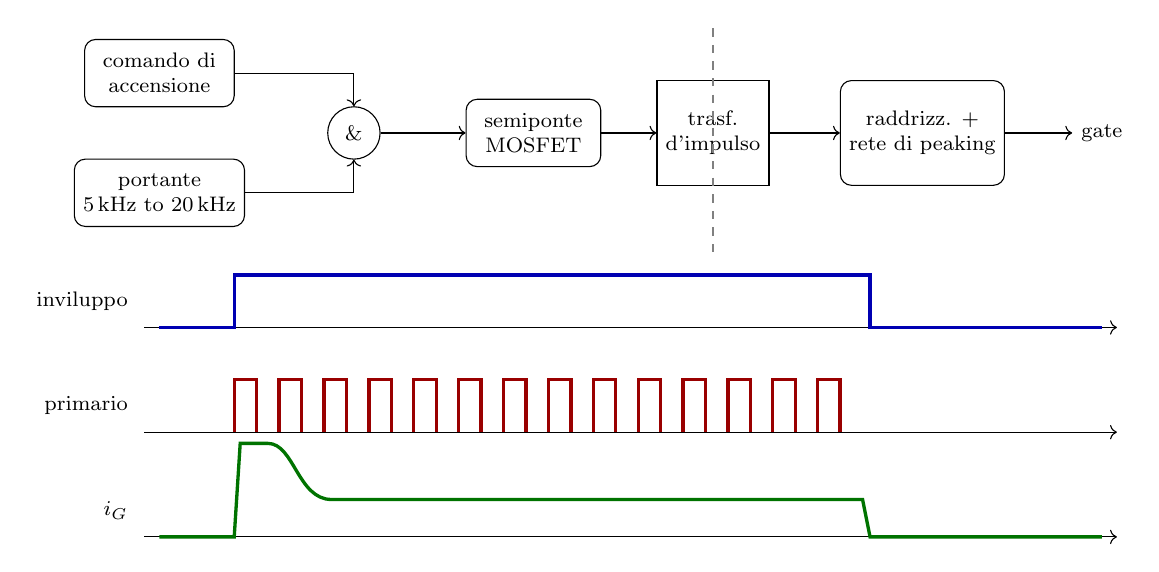
\begin{tikzpicture}[scale=0.95,transform shape]
  % block diagram
  \node[draw,rounded corners,minimum width=2.0cm,minimum height=0.9cm,align=center,font=\footnotesize]
    (cmd) at (0,0) {comando di\\accensione};
  \node[draw,rounded corners,minimum width=1.8cm,minimum height=0.9cm,align=center,font=\footnotesize]
    (osc) at (0,-1.6) {portante\\\SIrange{5}{20}{\kilo\hertz}};
  \node[draw,circle,minimum size=0.7cm,font=\footnotesize] (and) at (2.6,-0.8) {\&};
  \node[draw,rounded corners,minimum width=1.8cm,minimum height=0.9cm,align=center,font=\footnotesize]
    (drv) at (5.0,-0.8) {semiponte\\MOSFET};
  \node[draw,minimum width=1.0cm,minimum height=1.4cm,align=center,font=\footnotesize]
    (tr) at (7.4,-0.8) {trasf.\\d'impulso};
  \node[draw,rounded corners,minimum width=2.0cm,minimum height=1.4cm,align=center,font=\footnotesize]
    (rect) at (10.2,-0.8) {raddrizz. +\\rete di peaking};
  \node[font=\footnotesize] (th) at (12.6,-0.8) {gate};

  \draw[->] (cmd) -| (and);
  \draw[->] (osc) -| (and);
  \draw[->] (and) -- (drv);
  \draw[->] (drv) -- (tr);
  \draw[->] (tr) -- (rect);
  \draw[->] (rect) -- (th);
  \draw[dashed,gray] (7.4,0.6) -- (7.4,-2.4);

  % waveforms
  \begin{scope}[shift={(0,-3.4)}]
    \draw[->] (-0.2,0) -- (12.8,0);
    \node[font=\footnotesize,anchor=east] at (-0.3,0.35) {inviluppo};
    \draw[very thick,blue!70!black]
      (0,0) -- (1.0,0) -- (1.0,0.7) -- (9.5,0.7) -- (9.5,0) -- (12.6,0);
  \end{scope}
  \begin{scope}[shift={(0,-4.8)}]
    \draw[->] (-0.2,0) -- (12.8,0);
    \node[font=\footnotesize,anchor=east] at (-0.3,0.35) {primario};
    \foreach \x in {1.0,1.6,...,9.2} {
      \draw[very thick,red!60!black] (\x,0) -- (\x,0.7) -- (\x+0.3,0.7) -- (\x+0.3,0);
    }
  \end{scope}
  \begin{scope}[shift={(0,-6.2)}]
    \draw[->] (-0.2,0) -- (12.8,0);
    \node[font=\footnotesize,anchor=east] at (-0.3,0.35) {$i_G$};
    \draw[very thick,green!45!black]
      (0,0) -- (1.0,0) -- (1.08,1.25) -- (1.45,1.25)
      .. controls (1.8,1.25) and (1.85,0.5) .. (2.3,0.5)
      -- (9.4,0.5) -- (9.5,0) -- (12.6,0);
  \end{scope}
\end{tikzpicture}
\caption{Circuito B --- driver chopped. L'inviluppo di accensione è modulato da una
portante a \SIrange{5}{20}{\kilo\hertz}, così che il trasformatore gestisca solo i
volt$\cdot$secondo di un singolo periodo di portante. Un filtraggio leggero al
secondario ricostruisce una corrente di gate quasi continua.}
\label{fig:circB}
\end{figure}

Il filtraggio al secondario deve essere un compromesso: capacità sufficiente a
livellare il plateau tra gli impulsi di portante, ma non tanta da rallentare il
fronte di salita. Una disposizione comune è un raddrizzatore veloce che alimenta la
rete di peaking del Circuito~A, con un piccolo condensatore di filtro posto
\emph{a valle} della rete di peaking. Un primario a semiponte (o a ponte intero) è
preferibile a uno stadio single-ended, perché raddoppia l'escursione di flusso
utilizzabile e fornisce il reset intrinseco del nucleo.

\subsection{Circuito C --- Unità di gate in fibra ottica con generatore di corrente a due livelli}

Per apparecchiature in media tensione e per stack in serie, il comando viene
trasmesso su fibra ottica plastica e l'energia è immagazzinata localmente
(Fig.~\ref{fig:circC}). Lo stadio di uscita è una sorgente a due livelli: $M_1$
eroga l'impulso hard dal condensatore di accumulo $C_{st}$ attraverso la bassa
resistenza $R_1$; un monostabile rilascia poi $M_1$ e $M_2$ mantiene il plateau
attraverso $R_2$ per tutto il tempo in cui il comando ottico è presente. Tra un
impulso e l'altro $M_3$ applica la polarizzazione negativa e tiene il gate a bassa
impedenza.

\begin{figure}[htbp]
\centering
\begin{circuitikz}[american]
  % fibre receiver and logic
  \draw[->,very thick,orange!80!black] (0.0,4.4) -- (0.85,4.4);
  \node[font=\footnotesize,anchor=south] at (0.42,4.5) {POF};
  \node[draw,rounded corners,minimum width=2.6cm,minimum height=1.5cm,
        align=center,font=\footnotesize] (lg) at (2.2,4.4)
        {rx fibra\\formatore d'impulso\\+ monostabile};
  \draw[->,thick] (3.5,4.4) -- (4.6,4.4);
  \node[font=\scriptsize,anchor=south] at (4.05,4.78) {segnali di gate};
  % output stage boundary
  \draw[dashed,gray!70] (4.75,0.85) rectangle (13.85,7.45);
  \node[gray!50!black,font=\footnotesize,anchor=south west] at (4.85,0.95)
        {stadio di uscita --- flottante, riferito a K};
  % rails
  \draw (5.0,6.6) node[left,font=\small]{$+V_{cc}$} -- (11.9,6.6);
  \draw (5.3,6.6) to[C, l=$C_{st}$, *-] (5.3,1.6);
  \draw (5.3,1.6) -- (14.2,1.6);
  % M1 : hard pulse branch
  \node[pigfete, anchor=S] (M1) at (7.6,6.6) {};
  \draw (M1.D) to[R, l=$R_1$] (7.6,4.4);
  \draw (M1.G) -- ++(-0.4,0) node[left,font=\scriptsize]{hard};
  \node[font=\footnotesize,anchor=west] at (7.9,5.7) {$M_1$};
  % M2 : plateau branch
  \node[pigfete, anchor=S] (M2) at (9.9,6.6) {};
  \draw (M2.D) to[R, l=$R_2$] (9.9,4.4);
  \draw (M2.G) -- ++(-0.4,0) node[left,font=\scriptsize]{plateau};
  \node[font=\footnotesize,anchor=west] at (10.2,5.7) {$M_2$};
  % summing node
  \draw (7.6,4.4) -- (13.8,4.4);
  \fill (9.9,4.4) circle (1.6pt);
  \fill (11.6,4.4) circle (1.6pt);
  % M3 : off-state negative bias
  \node[nigfete, anchor=D] (M3) at (11.6,4.4) {};
  \draw (M3.S) -- (11.6,2.6);
  \draw (11.25,2.6) -- (11.95,2.6);
  \node[font=\footnotesize,anchor=north] at (11.6,2.5) {$-V_b$};
  \draw (M3.G) -- ++(-0.5,0) node[left,font=\scriptsize]{bias off};
  \node[font=\footnotesize,anchor=west] at (11.95,3.95) {$M_3$};
  % device-side network
  \draw (12.6,4.4) to[R, l_=$R_{GK}$, *-*] (12.6,1.6);
  \draw (13.4,4.4) to[zzD, *-*] (13.4,1.6);
  % thyristor
  \draw (14.2,6.9) node[above,font=\footnotesize]{A} -- (14.2,6.6);
  \draw (14.2,6.6) to[Ty, mirror, n=Th] (14.2,2.8);
  \draw (14.2,2.8) -- (14.2,1.0) node[below,font=\footnotesize]{K};
  \draw (Th.G) -| (13.8,4.4);
  \fill (14.2,1.6) circle (1.6pt);
\end{circuitikz}
\caption{Circuito C --- unità di gate in fibra ottica con accumulo locale e stadio di
uscita a due livelli. $M_1$ eroga l'impulso hard attraverso $R_1$, $M_2$ il back
porch attraverso $R_2$ e $M_3$ applica la polarizzazione negativa di riposo.}
\label{fig:circC}
\end{figure}

\paragraph{Note.}
\begin{itemize}
  \item $C_{st}$ deve essere di tipo a bassa ESL e collocato a pochi millimetri da
        $M_1$; è esso, e non l'alimentazione ausiliaria, a determinare il
        $\mathrm{d}i_G/\mathrm{d}t$ ottenibile.
  \item Il monostabile che termina l'impulso hard deve essere ritriggerabile e avere
        un tempo di conduzione massimo definito, così che un ingresso ottico bloccato
        alto non possa far superare $P_{G(AV)}$.
  \item Un watchdog sul collegamento ottico è indispensabile: la perdita della fibra
        deve essere interpretata come ``non accendere'', mai come ``accendi''.
        Conviene usare una portante ottica modulata anziché un livello luminoso
        statico, così da distinguere una fibra interrotta da un comando
        permanentemente disattivo.
\end{itemize}

\subsection{Circuito D --- Unità di gate autoalimentata}

Dove sul lato flottante non è disponibile alcuna alimentazione ausiliaria ---
tipicamente negli stack serie in alta tensione --- l'unità di gate preleva la propria
energia dalla tensione anodo--catodo (Fig.~\ref{fig:circD}). Una rete limitatrice di
corrente in alta tensione, in parallelo allo snubber, carica il condensatore di
accumulo locale durante l'intervallo di blocco; un regolatore shunt limita la
tensione di accumulo. La fibra trasporta solo il comando.

\begin{figure}[htbp]
\centering
\begin{circuitikz}[american]
  % ---------- rails ----------
  \draw (2.0,4.6) -- (10.6,4.6);
  \node[font=\footnotesize,anchor=south] at (5.9,4.65) {$+V_{cc}$};
  \draw (2.0,1.4) -- (13.2,1.4);
  % ---------- fibre receiver and logic ----------
  \draw[->,very thick,orange!80!black] (0.4,3.0) -- (2.1,3.0);
  \node[font=\footnotesize,anchor=south] at (1.25,3.1) {POF};
  \node[draw,rounded corners,minimum width=2.2cm,minimum height=1.3cm,
        align=center,font=\footnotesize] (lg) at (3.2,3.0) {rx fibra\\+ logica};
  \draw (3.2,3.65) -- (3.2,4.6);
  \draw (3.2,2.35) -- (3.2,1.4);
  \draw[->,dashed,gray!60!black] (4.3,3.0) -- (8.9,3.0);
  % ---------- storage and shunt regulator ----------
  \draw (6.8,4.6) to[zD, invert, *-*] (6.8,1.4);
  \node[font=\footnotesize,anchor=south east] at (6.7,3.75) {$D_{sh}$};
  \draw (8.2,4.6) to[C, *-*] (8.2,1.4);
  \node[font=\footnotesize,anchor=south east] at (8.1,3.75) {$C_{st}$};
  % ---------- output stage ----------
  \node[draw,rounded corners,minimum width=2.4cm,minimum height=1.2cm,
        align=center,font=\footnotesize] (out) at (10.2,3.0) {stadio di uscita\\a due livelli};
  \draw (10.2,3.6) -- (10.2,4.6);
  \draw (10.2,2.4) -- (10.2,1.4);
  % ---------- harvesting branch ----------
  \draw (13.2,6.8) -- (10.6,6.8);
  \draw (10.6,6.8) to[R, l_=$R_h$] (10.6,5.6);
  \draw (10.6,5.6) to[D, l_=$D_h$] (10.6,4.6);
  % ---------- gate network ----------
  \draw (11.4,3.0) -- (12.0,3.0) -- (12.0,4.4) -- (12.6,4.4);
  \draw (12.6,4.4) to[R, *-*] (12.6,1.4);
  \node[font=\footnotesize,anchor=east] at (12.3,2.5) {$R_{GK}$};
  % ---------- thyristor ----------
  \draw (13.2,7.3) node[above,font=\footnotesize]{A} -- (13.2,6.8);
  \draw (13.2,6.8) to[Ty, mirror, n=Th] (13.2,3.0);
  \draw (13.2,3.0) -- (13.2,0.9) node[below,font=\footnotesize]{K};
  \draw (Th.G) -| (12.6,4.4);
  \fill (13.2,6.8) circle (1.6pt);
  \fill (13.2,1.4) circle (1.6pt);
  % ---------- snubber ----------
  \draw (13.2,6.8) -- (14.6,6.8);
  \draw (14.6,6.8) to[R, l=$R_{sn}$] (14.6,4.8);
  \draw (14.6,4.8) to[C, l=$C_{sn}$] (14.6,2.0);
  \draw (14.6,2.0) -- (13.2,2.0);
  \fill (13.2,2.0) circle (1.6pt);
\end{circuitikz}
\caption{Circuito D --- unità di gate autoalimentata. L'energia è prelevata dalla
tensione di blocco anodo--catodo tramite $R_h$/$D_h$ e immagazzinata in $C_{st}$,
limitata dal regolatore shunt $D_{sh}$. Nessuna alimentazione ausiliaria attraversa
la barriera di isolamento.}
\label{fig:circD}
\end{figure}

\paragraph{Note.}
\begin{itemize}
  \item L'avviamento va gestito esplicitamente: la prima accensione dopo
        l'energizzazione può avvenire solo quando $C_{st}$ è carico. O il controllo
        attende un segnale di ``pronto'', oppure i primi cicli vanno accesi in una
        modalità che non richieda la piena energia di gate.
  \item $R_h$ dissipa in permanenza nello stato di blocco e va dimensionata per la
        piena tensione di picco ripetitiva. Prelevare energia dalla corrente dello
        snubber anziché da un partitore resistivo è nettamente più efficiente.
  \item In uno stack serie la rete di prelievo fa parte del progetto della
        ripartizione statica e dinamica della tensione e va inclusa nel relativo
        calcolo.
\end{itemize}

%======================================================================
\section{Protezioni, Layout ed EMC}
%======================================================================

\subsection{Protezioni a livello di componente}

\begin{itemize}
  \item \textbf{$R_{GK}$ sul dispositivo.} Obbligatoria. Va montata sui morsetti del
        dispositivo, non sulla scheda del driver.
  \item \textbf{Protezione contro la tensione inversa.} Un diodo serie o un diodo
        antiparallelo limita l'escursione negativa di gate. Una $V_{RGM}$ di pochi
        volt viene facilmente superata dalle oscillazioni in un cavo di gate lungo.
  \item \textbf{TVS bidirezionale} tra gate e catodo, sul dispositivo, per i
        transitori accoppiati nel loop di gate. La sua tensione di clamp deve stare
        tra la tensione di pilotaggio e $V_{FGM}$/$V_{RGM}$.
  \item \textbf{Resistenza serie di gate.} Oltre a fissare il livello di corrente,
        smorza la risonanza tra l'induttanza del loop di gate e la capacità di gate
        del dispositivo, impedendo ri-inneschi oscillatori.
  \item \textbf{Limitazione di corrente o fusibile allo stadio di uscita} lato
        driver, così che un cavo di gate in cortocircuito non distrugga l'unità di
        gate.
\end{itemize}

\subsection{Layout del loop di gate}

\begin{itemize}
  \item Usare un \textbf{doppino intrecciato} per il collegamento gate--catodo;
        doppino schermato, con schermo collegato solo dal lato driver, se l'ambiente
        è severo. Entrambi i conduttori devono seguire lo stesso percorso per tutta
        la lunghezza --- un errore comune è prelevare il ritorno di catodo da un
        morsetto di potenza.
  \item Mantenere minima l'\textbf{area del loop}. Il loop di gate è un'antenna
        ricevente per il $\mathrm{d}i/\mathrm{d}t$ del circuito principale.
  \item Mantenere la \textbf{lunghezza del cavo} entro il budget della
        Eq.~\eqref{eq:lloop}. Sotto \SI{1}{\metre} è preferibile; oltre qualche metro
        la rete di peaking va riprogettata o la tensione di pilotaggio aumentata.
  \item \textbf{Instradare il cavo di gate lontano dalle barre principali} e
        incrociarle ad angolo retto dove l'incrocio è inevitabile.
  \item In un ponte, mantenere il \textbf{ritardo di propagazione allineato} tra
        tutti i canali; un disallineamento si traduce direttamente in ripartizione
        disuniforme della tensione nelle connessioni serie e della corrente in quelle
        parallelo.
\end{itemize}

\subsection{Considerazioni di modo comune}

La capacità di barriera $C_{io}$ e il $\mathrm{d}v/\mathrm{d}t$ di commutazione
definiscono una corrente di modo comune che rientra attraverso la massa di
controllo. Misure di progetto: schermo elettrostatico nel trasformatore di
isolamento collegato alla massa di controllo; induttori di modo comune sui
conduttori primari; fibra ottica dove il $\mathrm{d}v/\mathrm{d}t$ è severo. La
verifica va fatta per misura diretta con un generatore di transitori di modo comune,
non per calcolo.

%======================================================================
\section{Diagnostica e Retroazione}
%======================================================================

Nelle apparecchiature industriali ci si attende che l'unità di gate fornisca almeno:

\begin{itemize}
  \item \textbf{Conferma dell'impulso} --- un segnale di ritorno che indica che
        l'impulso di corrente di gate è effettivamente circolato, ottenuto da un
        piccolo trasformatore di corrente o da uno shunt nel loop di gate. Permette
        di distinguere un guasto del driver da un guasto del dispositivo.
  \item \textbf{Monitoraggio della tensione di anodo} --- un partitore che indica se
        il dispositivo è in blocco o in conduzione. Serve per la verifica
        dell'accensione, per rilevare un dispositivo in corto prima
        dell'energizzazione e per la rilevazione di impulsi mancanti.
  \item \textbf{Blocco per sottotensione di alimentazione} --- inibisce l'accensione
        quando l'alimentazione locale è sotto il livello necessario a rispettare la
        specifica di pilotaggio. Accendere con corrente di gate insufficiente è più
        dannoso che non accendere affatto, perché l'accensione avviene su un'area
        ridotta.
  \item \textbf{Sovratemperatura e watchdog} sull'unità di gate stessa.
\end{itemize}

Per gli stack in serie, i segnali di conferma impulso di tutti i livelli andrebbero
combinati in un'unica indicazione di ``stack integro'', poiché un singolo impulso
mancante impone l'intera tensione dello stack su un solo dispositivo.

%======================================================================
\section{Esempio Numerico}
%======================================================================

Si consideri un grande tiristore press-pack a controllo di fase, all'incirca
\SI{6.5}{\kilo\volt}/\SI{2.6}{\kilo\ampere}, in un ponte esafase commutato dalla
rete con carico induttivo. Valori di datasheet rappresentativi (da sostituire con
quelli effettivi):

\begin{center}
\begin{tabular}{@{}lll@{}}
\toprule
$I_{GT}$ a \SI{25}{\celsius} & \SI{250}{\milli\ampere} & max \\
$I_{GT}$ a \SI{-40}{\celsius} & \SI{600}{\milli\ampere} & stimato, $\approx 2.5\times$ \\
$V_{GT}$ & \SI{3}{\volt} & max \\
$V_{GD}$ / $I_{GD}$ a $T_{vj,\max}$ & \SI{0.25}{\volt} / \SI{10}{\milli\ampere} & \\
$I_L$ & \SI{2}{\ampere} & \\
$V_{FGM}$ / $I_{FGM}$ / $V_{RGM}$ & \SI{10}{\volt} / \SI{8}{\ampere} / \SI{5}{\volt} & \\
$P_{GM}$ / $P_{G(AV)}$ & \SI{100}{\watt} / \SI{15}{\watt} & \\
\bottomrule
\end{tabular}
\end{center}

\paragraph{Passo 1 --- Ampiezza dell'impulso.}
Dalla Eq.~\eqref{eq:amp} con $I_{GT}(T_{\min}) = \SI{0.6}{\ampere}$ e un fattore 5:
$I_{G,\text{peak}} = \SI{3}{\ampere}$, ampiamente sotto $I_{FGM}$. Potenza di gate di
picco $\approx \SI{5}{\volt}\times\SI{3}{\ampere} = \SI{15}{\watt}$, ben sotto
$P_{GM}$.

\paragraph{Passo 2 --- Plateau.}
$I_{G,\text{plat}} = 1.5\times I_{GT}(\SI{25}{\celsius}) \approx
\SI{0.9}{\ampere}$. Con un intervallo di conduzione di \SI{6.7}{\milli\second} a
\SI{50}{\hertz}, il duty su una finestra di \SI{20}{\milli\second} è $1/3$, quindi
$P_{G(AV)} \approx \SI{3.5}{\volt}\times\SI{0.9}{\ampere}\times 1/3 \approx
\SI{1.1}{\watt}$, accettabile.

\paragraph{Passo 3 --- Rete di peaking.}
Si assuma $V_{drive} = \SI{15}{\volt}$ e $V_{GT}+V_{D} = \SI{3.5}{\volt}$, quindi
sono disponibili \SI{11.5}{\volt}. Dalla Eq.~\eqref{eq:peak}:
\[
  R_s = \frac{\SI{11.5}{\volt}}{\SI{3}{\ampere}} \approx \SI{4}{\ohm},
  \qquad
  R_s + R_p = \frac{\SI{11.5}{\volt}}{\SI{0.9}{\ampere} + \SI{0.11}{\ampere}}
  \approx \SI{11.4}{\ohm} \Rightarrow R_p \approx \SI{7.5}{\ohm},
\]
dove \SI{0.11}{\ampere} è la corrente deviata da $R_{GK} = \SI{27}{\ohm}$ a
\SI{3}{\volt}. Per una durata dell'impulso hard di \SI{20}{\micro\second}:
\[
  \tau_p = \frac{t_{hard}}{3} \approx \SI{6.7}{\micro\second},
  \qquad
  C_p = \frac{\tau_p}{R_p \parallel R_s}
      = \frac{\SI{6.7}{\micro\second}}{\SI{2.6}{\ohm}} \approx \SI{2.6}{\micro\farad}
      \;\rightarrow\; \SI{2.2}{\micro\farad}.
\]

\paragraph{Passo 4 --- Induttanza del loop di gate.}
Richiedendo $\mathrm{d}i_G/\mathrm{d}t = \SI{3}{\ampere\per\micro\second}$ e usando
la Eq.~\eqref{eq:lloop} con gli \SI{11.5}{\volt} pieni disponibili a $t=0^+$:
\[
  L_{loop} \le \frac{\SI{11.5}{\volt}}{\SI{3}{\ampere\per\micro\second}}
  \approx \SI{3.8}{\micro\henry}.
\]
A \SI{1}{\micro\henry\per\metre} per un doppino intrecciato, e riservando
\SI{1.5}{\micro\henry} alla dispersione del trasformatore e al layout, il cavo è
limitato a circa \SI{2}{\metre}. Tratte più lunghe richiedono una tensione di
pilotaggio maggiore oppure un'unità di gate locale.

\paragraph{Passo 5 --- Nucleo del trasformatore.}
Per un impulso trasmesso direttamente di \SI{500}{\micro\second} a \SI{24}{\volt} con
$N_1 = 20$ e $\Delta B = \SI{0.3}{\tesla}$, la Eq.~\eqref{eq:volt-sec} dà
$A_e \ge \SI{2000}{\milli\metre\squared}$ --- impraticabile. Spezzettando a
\SI{20}{\kilo\hertz} con duty al \SI{50}{\percent} il requisito scende a
$A_e \ge \SI{100}{\milli\metre\squared}$, un normale nucleo di piccole dimensioni.
Questo singolo calcolo è la ragione per cui il Circuito~B è la scelta standard ogni
volta che servono impulsi lunghi.

%======================================================================
\section{Checklist di Progetto}
%======================================================================

\begin{enumerate}
  \item Limiti di datasheet raccolti: $I_{GT}$, $V_{GT}$ a $T_{vj,\min}$;
        $V_{GD}$, $I_{GD}$ a $T_{vj,\max}$; $I_L$, $I_H$; $V_{FGM}$, $I_{FGM}$,
        $V_{RGM}$; $P_{GM}$, $P_{G(AV)}$.
  \item Retta di carico del driver tracciata sul diagramma di innesco e verificata a
        entrambi gli estremi di temperatura.
  \item $I_{G,\text{peak}}$ e $\mathrm{d}i_G/\mathrm{d}t$ coerenti con le condizioni
        in cui è specificato il valore di $\mathrm{d}i/\mathrm{d}t$.
  \item Durata dell'impulso verificata nel caso peggiore: minima corrente di carico,
        massima induttanza di carico, minima tensione di alimentazione.
  \item $P_{G(AV)}$ verificata alla massima frequenza di accensione e al massimo
        angolo di conduzione.
  \item Condizione di interdizione verificata: $V_{GK} < V_{GD}$ a $T_{vj,\max}$,
        con $R_{GK}$ montata.
  \item $V_{RGM}$ verificata comprese le oscillazioni, misurata sul dispositivo.
  \item Isolamento: distanze superficiali e in aria, tenuta a impulso, scariche
        parziali, $C_{io}$ e CMTI.
  \item Capacità volt$\cdot$secondo del trasformatore verificata alla massima
        larghezza d'impulso, massima tensione di alimentazione e massima temperatura;
        meccanismo di reset del nucleo presente.
  \item Budget di induttanza del loop di gate verificato rispetto alla lunghezza del
        cavo.
  \item Blocco per sottotensione, watchdog e interpretazione fail-safe della perdita
        del comando.
  \item Ritardo e jitter tra canali misurati, non supposti.
  \item Verifica eseguita sul dispositivo reale alla minima temperatura specificata,
        con l'alimentazione più debole prevista e con la corrente di gate misurata
        \emph{ai morsetti del dispositivo}.
\end{enumerate}

%======================================================================
\section*{Note sulla Verifica}
\addcontentsline{toc}{section}{Note sulla Verifica}
%======================================================================

Due prassi di misura meritano di essere esplicitate:

\begin{itemize}
  \item Misurare la corrente di gate con una sonda di corrente posta sul conduttore
        di gate \emph{al dispositivo}, e la tensione di gate in modo differenziale
        \emph{ai morsetti del dispositivo}. Ciò che fa l'uscita del driver è di
        interesse secondario; l'induttanza del loop e il cavo fanno parte del
        circuito.
  \item Provare agli estremi, non al nominale. Un driver di gate che funziona sul
        banco a \SI{25}{\celsius} con un dispositivo nuovo e un collegamento corto
        dice pochissimo sul comportamento a \SI{-25}{\celsius}, con un dispositivo di
        caso peggiore e la lunghezza di cavo installata. La maggior parte dei
        problemi di mancata accensione in campo si riconduce a uno di questi tre
        margini.
\end{itemize}

%======================================================================
\begin{thebibliography}{9}
\bibitem{iec60747} IEC 60747-6, \emph{Semiconductor devices --- Discrete devices
--- Part 6: Thyristors}, International Electrotechnical Commission.

\bibitem{iec60664} IEC 60664-1, \emph{Insulation coordination for equipment within
low-voltage supply systems --- Part 1: Principles, requirements and tests}.

\bibitem{semikron} A.~Wintrich, U.~Nicolai, W.~Tursky, T.~Reimann,
\emph{Application Manual Power Semiconductors}, 2nd ed., SEMIKRON International,
2015.

\bibitem{mohan} N.~Mohan, T.~M.~Undeland, W.~P.~Robbins, \emph{Power Electronics:
Converters, Applications and Design}, 3rd ed., Wiley, 2003.

\bibitem{baliga} B.~J.~Baliga, \emph{Fundamentals of Power Semiconductor Devices},
2nd ed., Springer, 2019.

\bibitem{blicher} A.~Blicher, \emph{Thyristor Physics}, Springer-Verlag, 1976.

\bibitem{rashid} M.~H.~Rashid (Ed.), \emph{Power Electronics Handbook}, 4th ed.,
Butterworth-Heinemann, 2018.
\end{thebibliography}

\end{document}
